%%%%%%%%%%%%%%%%%%%%%%%%%%%%%%%%%%%%%%%%%%%%%%%%%%%%%%%%%%%%%%%%%%%%%%%%%%%%%%%%
%2345678901234567890123456789012345678901234567890123456789012345678901234567890
%        1         2         3         4         5         6         7         8

\documentclass[letterpaper, 10 pt, conference]{ieeeconf}  % Comment this line out
                                                          % if you need a4paper
%\documentclass[a4paper, 10pt, conference]{ieeeconf}      % Use this line for a4
                                                          % paper
\IEEEoverridecommandlockouts                              % This command is only
                                                          % needed if you want to
                                                          % use the \thanks command
%\overrideIEEEmargins
% See the \addtolength command later in the file to balance the column lengths
% on the last page of the document

% The following packages can be found on http:\\www.ctan.org
\usepackage{cite}
\usepackage{amsmath,amssymb,amsfonts}
\usepackage{algorithmic}
\usepackage[ruled,vlined,linesnumbered]{algorithm2e}
\usepackage{graphicx}
\usepackage{textcomp}
\usepackage{xcolor}
\usepackage{flowchart}
\usetikzlibrary{shapes,arrows}

\title{\LARGE \bf
Outlier Detection for ARM Data
}

\author{Yuping Lu$^{1}$, Jitendra Kumar$^{2}$, Nathan Collier$^{2}$ and Michael A. Langston$^{1}$% <-this % stops a space
\thanks{$^{1}$University of Tennessee, Knoxville, TN, USA}%
\thanks{$^{2}$Oak Ridge National Laboratory, Oak Ridge, TN, USA}%
}

\begin{document}
\maketitle
\thispagestyle{empty}
\pagestyle{empty}

%%%%%%%%%%%%%%%%%%%%%%%%%%%%%%%%%%%%%%%%%%%%%%%%%%%%%%%%%%%%%%%%%%%%%%%%%%%%%%%%
\begin{abstract}

The Atmospheric Radiation Measurement (ARM) Data Center collects data from either permanent or mobile facilities around the globe. These data are then ingested and used to create high level scientific products which requires great accuracy. Multiple methods are available to detect these outliers from ARM time series data. As outliers are common in the collected data which could be either an instrument failure or extreme weather event, Pearson Correlation Coefficient was first examined to measure the pairwise correlations between variables. New version of Singular Spectrum Analysis (SSA) was also introduced to detect outliers. K-means was applied in a different manner to filter out the abnormal records as well. Pearson Correlation Coefficient, SSA and K-means methods were later combined together as a whole framework to track down these outliers. Compared to the current data quality reports stored in the DQR database, our results showed this framework is promising.

\end{abstract}


%%%%%%%%%%%%%%%%%%%%%%%%%%%%%%%%%%%%%%%%%%%%%%%%%%%%%%%%%%%%%%%%%%%%%%%%%%%%%%%%
\section{Introduction}
The Atmospheric Radiation Measurement (ARM) user facility was founded by the U.S. Department of Energy (DOE) in 1989 \cite{ARM}. Since then, its aim is to be the platforms for the observation and study of Earth's climate. Huge ARM datasets are collected from instruments deployed in different ground stations across the globe \cite{stokes1994atmospheric}. ARM Data Center is responsible for ingesting these collected data and creates high level scientific data products for distribution and the improvement of global climate models (GCMs) \cite{gaustad2014scientific}. These high level data products, also called "Value Added Products" (VAPs) are highly dependent on the correctness of the raw data. Thus it is crucial to detect those outliers in the raw data and correct them.

As outliers are pretty common in these datasets. Currently, these datasets are checked manually and outliers are stored in Data Quality Report (DQR) database to be fixed. 

We will use this section to introduce the background of outlier detection for time series data. \cite{gupta2014outlier} 


\section{Datasets}
ARM data are stored in Network Common Data Form (NetCDF) format which is self-describing and machine-independent \cite{rew1990netcdf, NetCDF}. NetCDF format also has good performance and data compression. It is commonly used to handle scientific data, especially those from the climatology, meteorology, oceanography and GIS projects. ARM data is publicly available and can be downloaded from ARM Data Archive (http://www.archive.arm.gov). Kinds of raw data are stored in ARM Data Center. It ranges from \textit{Atmospheric Profiling} to \textit{Satellite Observations}. All these data are measured at different locations using different instruments. Each instrument may only work on a specified time range. For the raw NetCDF dataset collected from each instrument, it contains multiple variables. 

\begin{table}[ht]
\caption{SGPMET datasets tested}
\label{tab:datasets}
\centering
\begin{tabular}{|l|c|c|c|c|c|c|c|c|}
\hline
Instrument & E1 & E3 & E4 & E5 & E6 & E7\\
Begin Year & 1996 & 1997 & 1996 & 1997 & 1997 & 1996\\
End Year & 2008 & 2008 & 2010 & 2008 & 2010 & 2011\\
\hline
Instrument & E8 & E9 & E11 & E13 & E15 & E20\\
Begin Year & 1994 & 1994 & 1996 & 1994 & 1994 & 1994\\
End Year & 2008 & 2017 & 2017 & 2017 & 2017 & 2010\\
\hline
Instrument & E21 & E24 & E25 & E27 & E31 & E32\\
Begin Year & 2000 & 1996 & 1997 & 2004 & 2012 & 2012\\
End Year & 2017 & 2008 & 2001 & 2009 & 2017 & 2017\\
\hline
Instrument & E33 & E34 & E35 & E36 & E37 & E38\\
Begin Year & 2012 & 2012 & 2012 & 2012 & 2012 & 2012\\
End Year & 2017 & 2017 & 2017 & 2017 & 2017 & 2017\\
\hline
\end{tabular}
\end{table}

In this paper, we only tested Surface Meteorology Systems (MET) data collected from the Southern Great Plains (SGP). There were total 24 instruments in SGP area and we chose 5 typical variables which are \textit{temp\_mean}, \textit{vapor\_pressure\_mean}, \textit{atmos\_pressure}, \textit{rh\_mean} and \textit{wspd\_arith\_mean} from multiple variables. Table 1 contains the detail of these datasets. 

\section{Methodology}
We have introduced many kinds of outlier detection method in the first section. We carefully picked three algorithms and tested them on ARM data. We also did necessary preprocessing before running these algorithms. The first level raw data is stored in minute level. It is normalized for pairwise comparison algorithm. Some algorithms may not need so much detail information to extract outliers. Thus we created a second level data by averaging the 1440 minute data points into one day point from the raw data. The second level data can save a lot of running time and is easier for Plotly \cite{plotly} and Matplotlib \cite{Hunter:2007} to visualize. The third level data was especially created for multivariate method by standardization all the 5 variables into the same scale based on the second level data. Below we will talk about each algorithm in detail. 

\subsection{Pearson Correlation Coefficient} 
Pearson Correlation Coefficient was first introduced by Karl Pearson\cite{pearson1895note}. It is used to measure the linear correlation between two variables. Pearson correlation coefficient is calculated from the covariance of two variables divided by the multiplication of the standard deviation of those two variables. Thus the value falls in [-1, 1]. If the value is close to -1, it means those two variables are highly negatively related. On the other hand, then the two variables are strongly positively related. If the value is near 0, it means those two variables don't have linear relation. 

\begin{figure*}[ht]
    \centering
    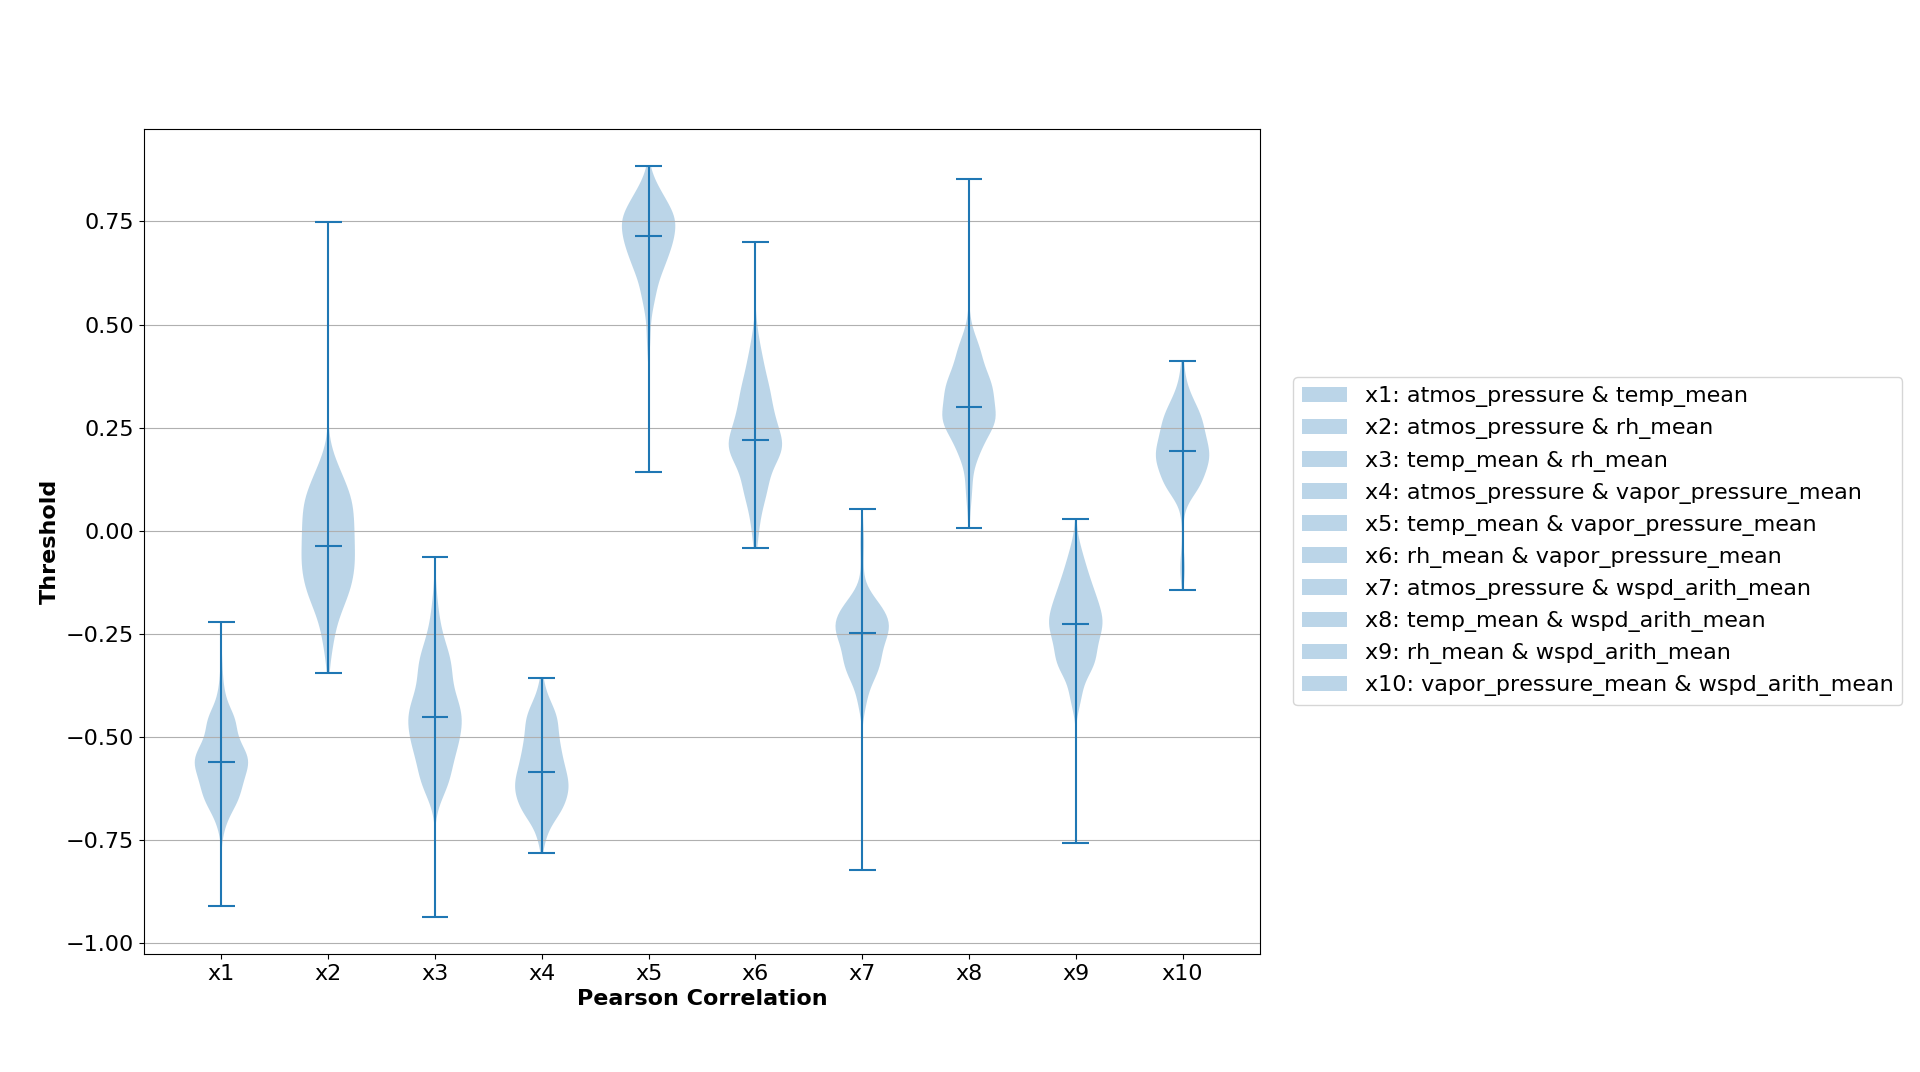
\includegraphics[width=\textwidth]{Spring.png}
    \caption{Violin plot: Spring 5 variables from SGPMET}
    \label{fig:pc}
\end{figure*}

We performed pairwise comparison of the 5 variables using Pearson Correlation on all the instruments in a seasonal level. The result in figure 1 makes sense and all the correlations in this violin plot are normally distributed. For example, x5 the Pearson Correlation between \textit{temp\_mean} and \textit{vapor\_pressure\_mean} is positively correlated with correlation mean close to 0.75. x1 is negatively correlated with correlation mean close to -0.60. We used this correlation as base knowledge. If a pairwise pearson correlation of two variables from a specific season of a instrument falls out of that range, we treated that seasonal data as outliers.
x1 is negatively correlated with correlation mean close to -0.60. We used this correlation as base knowledge. If a pairwise pearson correlation of two variables from a specific season of a instrument falls out of that range, we treated that seasonal data as outliers.

\subsection{Singular Spectrum Analysis}
Singular Spectrum Analysis (SSA) is a popular method for time series data analysis \cite{golyandina2013singular, golyandina2014basic}. The general idea is to use a subset of the decomposition of trajectory matrix to approximate it. Many applications can be found in \cite{golyandina2013singular}. For example, SSA can be applied to monitor volcanic activity \cite{bozzo2010relationship}. It can also be used to extract trend \cite{alexandrov2008method}. Different from the classic SSA method, we defined our own version of SSA to best work on ARM data. Figure 2 is a demonstration of the workflow of SSA. Below is the formal description of the algorithm.

% SSA workflow
\begin{figure}[ht]
    \centering
    % Define block styles
    \tikzstyle{decision} = [diamond, draw, fill=blue!20, text width=4.5em,text badly centered, node distance=3cm, inner sep=0pt]
    \tikzstyle{block} = [rectangle, draw, fill=blue!20, minimum width=5em, text centered, rounded corners, minimum height=2em]
    \tikzstyle{line} = [draw, -latex']
    \tikzstyle{cloud} = [draw, ellipse,fill=red!20, node distance=3cm, text width=3em, minimum height=2em]
    \begin{tikzpicture}[node distance = 2cm, auto]
        % Place nodes
        \node [block] (init) {\small Embedding};
        \node [block, right of=init, node distance=3cm] (decomp) {\small Decomposition};
        \node [block, below of=decomp] (freq) {\small Finding Dominant Frequency};
        \node [block, below of=freq] (period) {\small Converting Periodicity into Frequency};
        \node [block, below of=period] (approx) {\small Approximation};
        \node [block, left of=approx, node distance=3cm] (re) {\small Reconstruction};
        % Draw edges
        \path [line] (init) -- (decomp);
        \path [line] (decomp) -- (freq);
        \path [line] (freq) -- (period);
        \path [line] (period) -- (approx);
        \path [line] (approx) -- (re);
    \end{tikzpicture}
    \caption{Flowchart of SSA}
    \label{fig:pcs}
\end{figure}

\begin{figure*}[ht]
    \centering
    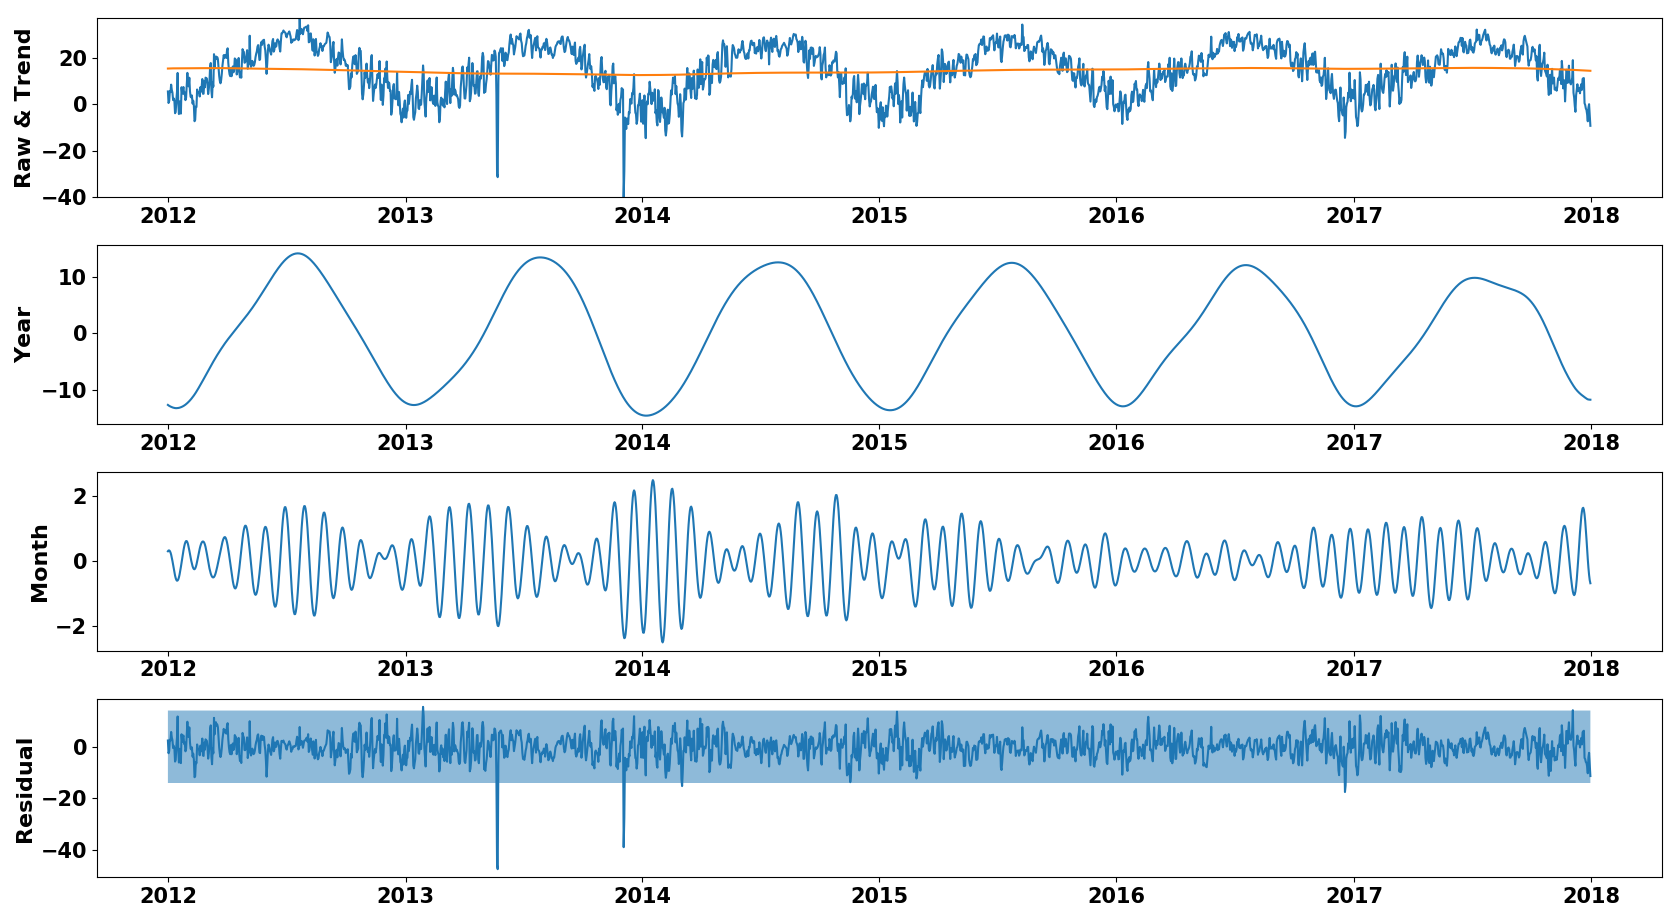
\includegraphics[width=\textwidth]{E33.png}
    \caption{Example of SSA application on ARM data. The full decomposition of temp\_mean data from instrument E33.}
    \label{fig:ssa}
\end{figure*}

% SSA algorithm description
% Needs Nate's help, especially step 3. Not sure how to describe this step accurately.
Assume we have an ARM time series data Y of length T.
\begin{align*}
Y =(y_1,\ \ldots,\ y_T)
\end{align*}
Here $T > 2$ and $y_i$ is not empty. Let $L\ (1 < L \leq T/2)$ be the window size and $K = T - L + 1$. In general, the algorithm contains two main parts: decomposition and reconstruction.

1) The first step is to form trajectory matrix \textbf{X} from vector Y by embedding subsets of Y. These subsets of Y $X_i$ are lagged vectors of length L.  
\begin{align*}
X_i = (y_i,\ \ldots,\ y_{L+i-1})^T \quad (1 \leq i \leq K) \\
\mathbf{X} = [X_i,\ \ldots,\ X_K] 
\end{align*}
Thus the trajectory matrix is
\begin{equation}
\mathbf{X} = (x_{ij})_{i,j=1}^{L,K}  = \left(\begin{IEEEeqnarraybox*}[][c]{,c/c/c/c/c,}
y_1 & y_2 & y_3 & \ldots & y_K\\
y_2 & y_3 & y_4 & \ldots & y_{K+1}\\
y_3 & y_4 & y_5 & \ldots & y_{K+2}\\
\vdots & \vdots & \vdots & \ddots & \vdots\\
y_L & y_{L+1} & y_{L+2} & \ldots & y_T
\end{IEEEeqnarraybox*}\right)
\end{equation}
where $x_{ij} = y_{i+j-1}$. We can see from equation 1 that matrix \textbf{X} has equal elements on anti-diagonals and therefore it is Hankel matrix.

2) Assume matrix $\mathbf{S}=\mathbf{XX}^T$, thus we perform the singular value decomposition (SVD) on $\mathbf{S}$. The eigenvalues of S are denoted by $\lambda_1, \ldots, \lambda_L$ in the decreasing order of magnitude $(\lambda_1 \geq \ldots \geq \lambda_L \geq 0)$ and corresponding eigenvectors are denoted by $P_1, \ldots, P_L$. Let $d = rank\ \mathbf{X}$ and $V_i = \mathbf{X}^T P_i / \sqrt{\lambda_i} (i = 1, \ldots, d)$. Thus, the trajectory matrix X can also be written as
\begin{equation}
\mathbf{X} = \mathbf{X_1} + \ldots + \mathbf{X_d}
\end{equation}
where $\mathbf{X_i} = \sqrt{\lambda_i} P_i V_i^T$.

3) In this step, we use Fast Fourier transform (FFT) to find the dominant frequency of each eigenvector \cite{cooley1965algorithm} . Algorithm 1 shows the whole process.

\begin{algorithm}[ht]
\DontPrintSemicolon
\SetAlgoLined
%\KwResult{Dominant frequency of each eigenvector}
\SetKwInOut{Input}{Input}
\SetKwInOut{Output}{Output}
\Input{$\lambda$ of $\mathbf{S}$ and corresponding eigenvectors $\mathbf{P}$}
\Output{Dominant frequency of each eigenvector}
\BlankLine

fftfreq $\leftarrow$ Discrete Fourier Transform sample frequencies\;
fft $\leftarrow$ Discrete Fourier Transform\;
len $\leftarrow$ size of $\lambda$\;
frequencies $\leftarrow$ zero vector of size len\;
fs $\leftarrow$ fftfreq($\lambda$)\;
ix $\leftarrow$ indices that sort fs\;
fs $\leftarrow$ fs[ix]\;
\For{i in range(len)}{
    p1 $\leftarrow$ abs(fft($\mathbf{P}$[:,i]))\;
    ps $\leftarrow$ p1**2\;
    ps $\leftarrow$ ps[ix]\;
    frequencies[i] $\leftarrow$ fs[index of the maximum value in ps]\;
}
\Return abs(frequencies)
\caption{Dominant Frequency Finder}
\end{algorithm}

4) Let G be the vector of user specified periodicity. We then convert G into a vector of targeted frequency TF for the next step. Here 0 is also added to TF. We use M to denote the length of TF.

5) As mentioned in step 2, there are d $\mathbf{X_i}$. The goal is to build an approximation of X by taking a subset of the decomposition $\mathbf{X_i}$. This approximation is formed by taking eigenvectors whose dominant frequency is close to the targeted frequency. Thus we have an approximation matrix $\mathbf{Xt}$ of size $M \times L \times K$.

6) Now we reconstruct the signal $\hat{Y}$ by taking a mean of all the approximations. The generated matrix $\mathbf{Yt}$ with size $M \times T$ can be used to approximate Y.

\begin{equation}
\hat{Y} =  \displaystyle\sum_{i=1}^{M} \mathbf{Yt}[i]
\end{equation}

In this paper, we chose the temp\_mean data from instrument E33 as Y to illustrate SSA. Because SSA requires the time series data to be continuous, we replaced the empty points with the average temp\_mean value for that day in a year. 

We set L = 400 and picked year and month as the periodicity groups G = [365, 30]. Thus TF = [0, 0.00273973, 0.03333333]. The generated matrix $\mathbf{Yt}$ has 3 rows after performing SSA. And $\hat{Y}$ = $\mathbf{Yt}[0]$ + $\mathbf{Yt}[1]$ + $\mathbf{Yt}[2]$. The residual is then extracted from the raw data R = Y - $\hat{Y}$. As $\hat{Y}$ is the approximation which is a "perfect" representation of Y. We then extracted the extreme values from the residual. Those extracted outliers are outliers. Figure 3 is a visualization of the result. The first row is the raw data Y. The orange line $\mathbf{Yt}[0]$ is the trend. As we can see, the trend is pretty flat from 2012 to 2017. The second row and third row are $\mathbf{Yt}[1]$, $\mathbf{Yt}[1]$ respectively. The Year data matches the pattern of the raw data. The last row is the residual. Those peak values outside the blue shaded area are outliers.

\subsection{K-means}
K-means is a partitioning clustering algorithm \cite{macqueen1967some, hartigan1979algorithm}. It starts with the k centroids user specified, and assigns the points to the nearest centroid. Then it computes new k centroids and assign the rest points to these centroids again. The process repeats until it converges. 

% K-means algorithm
\begin{algorithm}[ht]
\DontPrintSemicolon
\SetAlgoLined
%\KwResult{Dominant frequency of each eigenvector}
\SetKwInOut{Input}{Input}
\SetKwInOut{Output}{Output}
\Input{ARM time series data}
\Output{Outliers}
\BlankLine

outliers $\leftarrow \varnothing$\;
df $\leftarrow$ ARM time series data\;
data $\leftarrow$ df['atmos\_pressure','temp\_mean',\
'rh\_mean','vapor\_pressure\_mean','wspd\_arith\_mean']\;
number\_of\_clusters $\leftarrow$ 4\;
clusters $\leftarrow$ K-means(data, number\_of\_clusters)\;
distances $\leftarrow$ Distance between each point and its centroid\;
mean $\leftarrow$ arithmetic mean of distances\;
sigma $\leftarrow$ standard deviation of distances\;
threshold $\leftarrow$ mean + 3 * sigma\;
\For{i in range(size of distances)}{
    \If{distances[i] $>$ threshold}{
        outliers $\leftarrow$ outliers $\cup$ {distances[i]}
    }
}
\Return outliers
\caption{K-means Outlier Detection}
\end{algorithm}

In this paper, we didn't stop after clustering ARM data with K-means. We transformed the generated clusters into a vector of distance between each point and its corresponding centroid. Algorithm 2 describes the whole process. Unlike SSA, we used all the 5 variables mentioned in Datasets section together to extract outliers.

\begin{figure*}[ht]
    \centering
    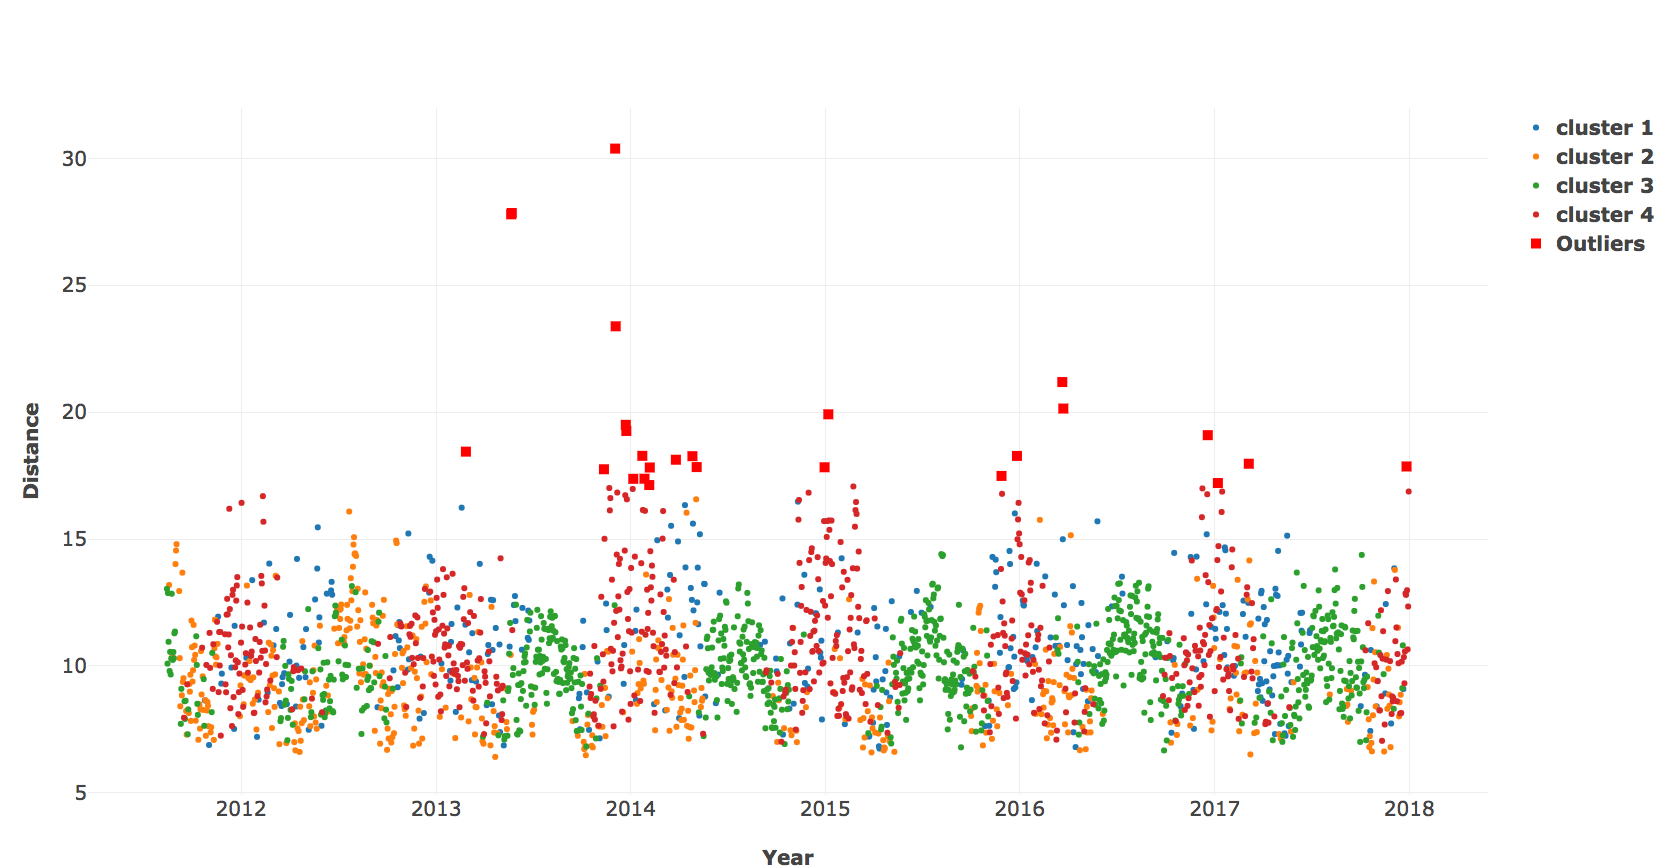
\includegraphics[width=\textwidth]{kmeans.png}
    \caption{Outliers detected using K-means for E33}
    \label{fig:kmeans}
\end{figure*}

Again, we used data from instrument E33 as an example for K-means. Here we set k to 4 as each year has 4 seasons.  Figure 4 visualized the outliers detected from E33. Y axes in this figure is the distance metric. The pattern of these points is close to the raw data.

\section{Results and Discussion}
% mention the usage of python and implementation?
SSA is an univariate method. K-means is a multivariate method. Results and pics go here. Comparison metric: DQR database \cite{mccord2016arm}. 

Add the drawbacks of each algorithm and their strong parts.

% add three sigma rule here
How do you pick extreme values as outliers? Some methods do not work. Here we use the three sigma rule to extract outliers \cite{pukelsheim1994three}.

Precision and recall was first defined in \cite{perry1955machine}. It is commonly used to measure the quality of classification tasks \cite{olson2008advanced}. Precision is calculated from True Positives divided by the sum of True Positives and False Positives. On the other hand, recall is measured from True Positives divided by the sum of True Positives and False Negatives. In this paper, detected outliers in the DQR database are the ground truth. So we treated these as True Positives. Thus detected outliers not in the DQR database are False Positives. Undetected values which in the DQR database are False Negatives, and which not in the DQR database are True Negatives. Analysis of table 2 and 3 goes here.

\begin{figure*}[ht]
    \centering
    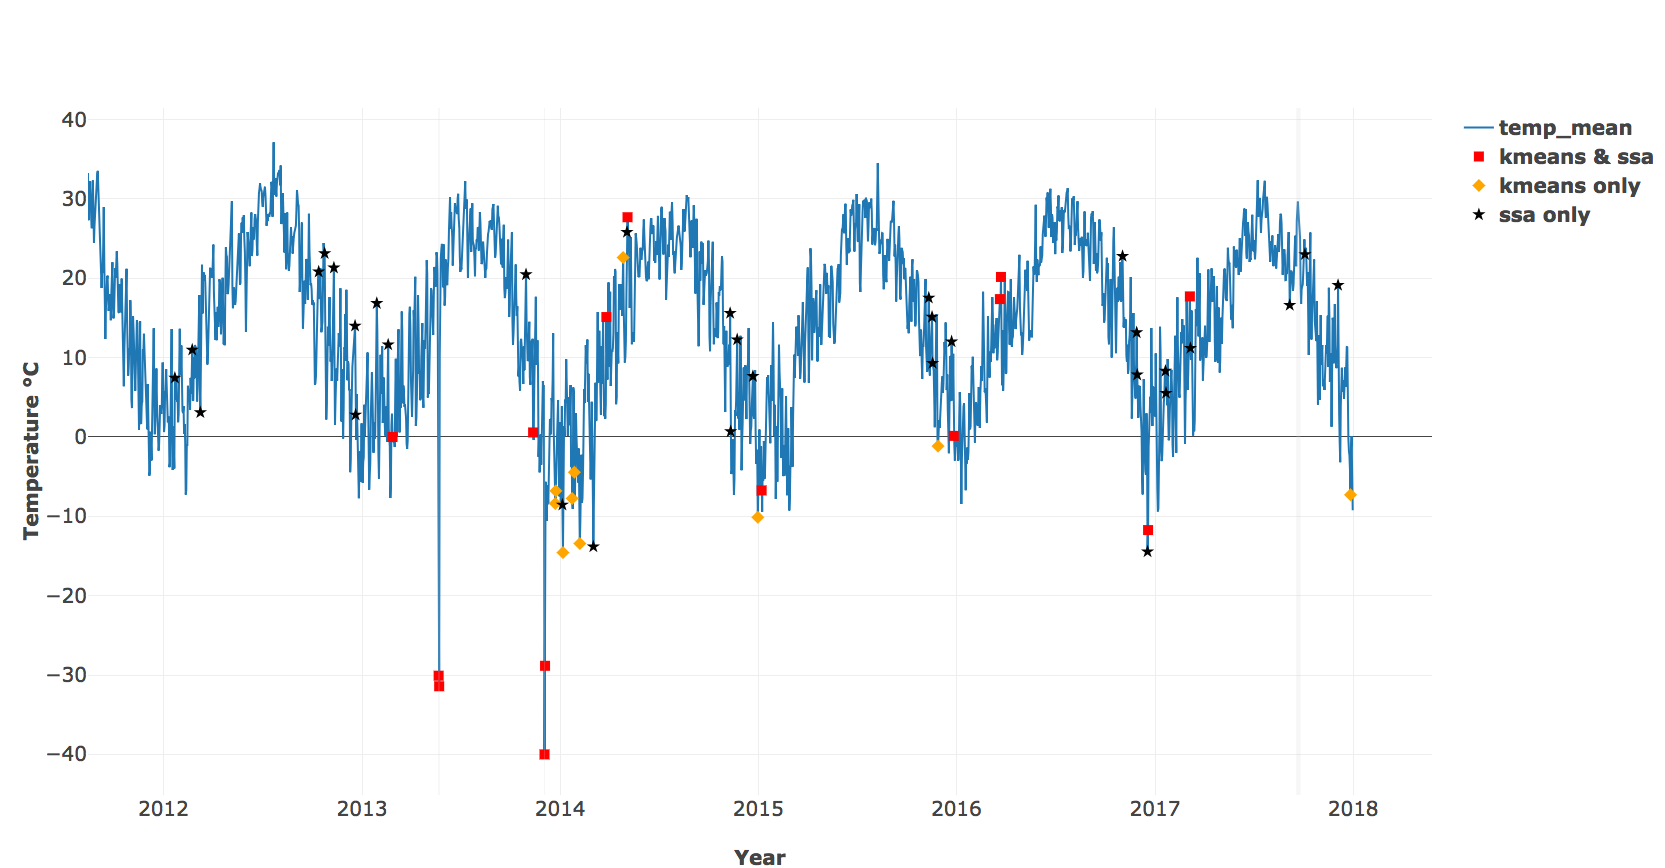
\includegraphics[width=\textwidth]{combined.png}
    \caption{E33 temp\_mean combined}
    \label{fig:combined}
\end{figure*}

\begin{table}[ht]
\caption{Precision and Recall of SSA and K-means}
\label{tab:pr}
\centering
\begin{tabular}{|l|c|c|c|}
\hline
Method & Variable & Precision & Recall\\
\hline
SSA & temp\_mean & 16.00\% & 1.20\%\\
SSA & vapor\_pressure\_mean & 20.70\% & 1.40\%\\
SSA & atmos\_pressure & 0.00\% & 0.00\%\\
SSA & rh\_mean & 14.80\% & 0.50\%\\
SSA & wspd\_arith\_mean & 0.60\% & 1.50\%\\
Kmeans & 5 together & 12.90\% & 1.90\%\\
Combined & 5 together & 11.10\% & 4.10\%\\
\hline
\end{tabular}
\end{table}

\begin{table}[ht]
\caption{Comparison of SSA and K-means Outlier Set Size}
\label{tab:comp}
\centering
\begin{tabular}{|l|c|}
\cline{2-2}
\multicolumn{1}{l|}{} & Outlier Set Size\\
\hline
SSA & 922\\
K-means & 508\\
Intersection & 378\\
Symmetric Difference & 674\\
\hline
\end{tabular}
\end{table}

More figures and results can be found on github. 
%https://github.com/YupingLu/arm-pearson 
%https://github.com/YupingLu/arm-ssa

\section{Conclusions}
After we compute those extreme values, use other methods to extract part of them as outliers?
We presented a combined model to detect outliers for ARM data. Future work: 
ML and tried methods working on multiple instruments multiple sites \cite{phillips2015graph}.

%\addtolength{\textheight}{-12cm}  % This command serves to balance the column lengths
                                  % on the last page of the document manually. It shortens
                                  % the textheight of the last page by a suitable amount.
                                  % This command does not take effect until the next page
                                  % so it should come on the page before the last. Make
                                  % sure that you do not shorten the textheight too much.

%%%%%%%%%%%%%%%%%%%%%%%%%%%%%%%%%%%%%%%%%%%%%%%%%%%%%%%%%%%%%%%%%%%%%%%%%%%%%%%%
\section*{Acknowledgment}
This research was supported by the Atmospheric Radiation Measurement (ARM) user 
facility, a U.S. Department of Energy (DOE) Office of Science user facility 
managed by the Office of Biological and Environmental Research.


\bibliography{main} 
\bibliographystyle{IEEEtran}


\end{document}